\section{Evaluation}
\label{sec:evaluation}

The utmost goal of our performance evaluation is two-fold: (i) measure the accuracy of our learning model in ranking Internet videos in order of \emph{hotness}, and (ii) evaluate the performance of our replication scheme in meeting viewers' expectations properly. Further details about evaluation set-up are available in Section\ref{sec:simulation_methodology}.

\subsection{Performance Evaluation Metrics}
\label{subsec:methodology_metrics}

We aim to evaluate the performance of two main WiseReplica modules: machine-learned ranking and replication strategy. Hence we group evaluation metrics as follows:

\subsubsection{Machine-Learned Ranking Accuracy} 

We adopt the normalized Discounted Cumulative Gain (nDCG) criterion as the main evaluation metric for our learning model. nDCG is a standard quality measure in information retrieval, especially for Web search~\cite{jarvelin2002cumulated}. The DCG definition is $DCG_{L}=\sum_{i=1}^L \frac{2^{F(i)}-1}{\log_{2}(1+i)}$, where $L$ is the global set of ranked videos, and $F(i)$ is the rank position of $i$th video. To compute nDCG, we divide DCG measure by the idealized DCG with perfect order of the set $L$. Thus, the perfect model scores $1$. Unlike typical information retrieval problems, as a ranking of web content, our model does not have the notion of \emph{query}. Instead, we rely on nDCG robustness to measure the performance of our learning model as a global ranking problem. Since the ranking problem shares properties with both classification and regression problems, we compare nDCG to other three popular machine learning metrics: the mean square error, a standard metric for regressions; precision, for classification; and a less robust, well-known variant of nDCG, namely  in this work nDCG(2). We evaluate three different state-of-the-art ensemble learning methods available in \textsc{Scikit-learn} library: \textsc{Random Forest}, \textsc{Extremely Randomized Trees}, and \textsc{Gradient Tree Boosting}. Moreover, we report briefly on the sample size for learning, number of estimators or learners of ensemble methods, measurements or features importance, and the computational overhead of our model, including memory usage and computation time for prediction.

\subsubsection{Metrics for Replication Strategies in Peer-Assisted VoD Systems} 

Assuming that content and CDN providers are committed to enforcing bitrate as main QoS metric through SLA contracts, we consider SLA violation as the primary performance metric. Thus, a SLA violation happens whenever the peer-assisted VoD system does not provide the minimum average bitrate for preventing rebuffering. This measures the WiseReplica capacity of meeting consumers' expectations. We also investigate the impact of our replication scheme using storage domains in peer-assisted VoD systems. To this end, our evaluation metrics are network and storage usage. Finally, we compare WiseReplica results with a non-collaborative caching and the Oracle-like assumption, described in Subsection~\ref{subsec:methodology_replication_schemes}. 

\subsection{Fitting and Measuring the Accuracy of Our Ranking Model}
\label{subsec:prediction_performance}

The evaluation of our learning model comprises: ensemble method selection, number of \emph{estimators},  sample size for leaning, and inputs' relative importance. In this subsection, we aim to evaluate the most important settings and tune our model towards higher accuracy, using the learning framework described in Subsection~\ref{subsec:framework}.

\subsubsection{Selecting and Fitting an Ensemble Method}

Ensemble methods have become very popular in statistical learning. Their algorithms combine several \emph{estimators} or \emph{week learners} to provide robust learning models and prevent overfitting. We fit and evaluate our model with three methods from \textsc{Scikit-learn} library: \textsc{Random Forest}(RF), \textsc{Extremely Randomized Trees}(ET), and \textsc{Gradient Tree Boosting}(GB). We consider two distinct samples with 124 thousand lines each, one for training and other for testing. We set to 10 the number of estimators as a common setting. All other parameters have default settings. Based on four metrics detailed on Subsection~\ref{subsec:methodology_metrics}, \textsc{Random Forest} fits our model better. Figure~\ref{fig:ensemble_method_eval} depicts three of these metrics. \textsc{Random Forest} performs particularly well in nDCG score, the main metric for ranking problems. While \textsc{Extremely Randomized Trees} and \textsc{Gradient Tree Boosting} score 0.9126 and 0.4128 respectively, \textsc{Random Forest} scores 0.9594. In terms of precision, \textsc{Random Forest} slightly better, with a score of 0.9922.  \textsc{Extremely Randomized Trees} scores 0.9899, and \textsc{Gradient Tree Boosting} scores 0.9502.  It also outperforms the other two methods regarding the mean square error metric, scoring 0.0094 compared to 0.0122 with \textsc{Extremely Randomized Trees} and 0.1021 with \textsc{Gradient Tree Boosting}. nDCG(2) metric confirms these results. Therefore, we select \textsc{Random Forest} method for our ranking model and nDCG as the key accuracy metric. 

\begin{figure}[htbp]
	\begin{minipage}[t]{0.48\linewidth}
     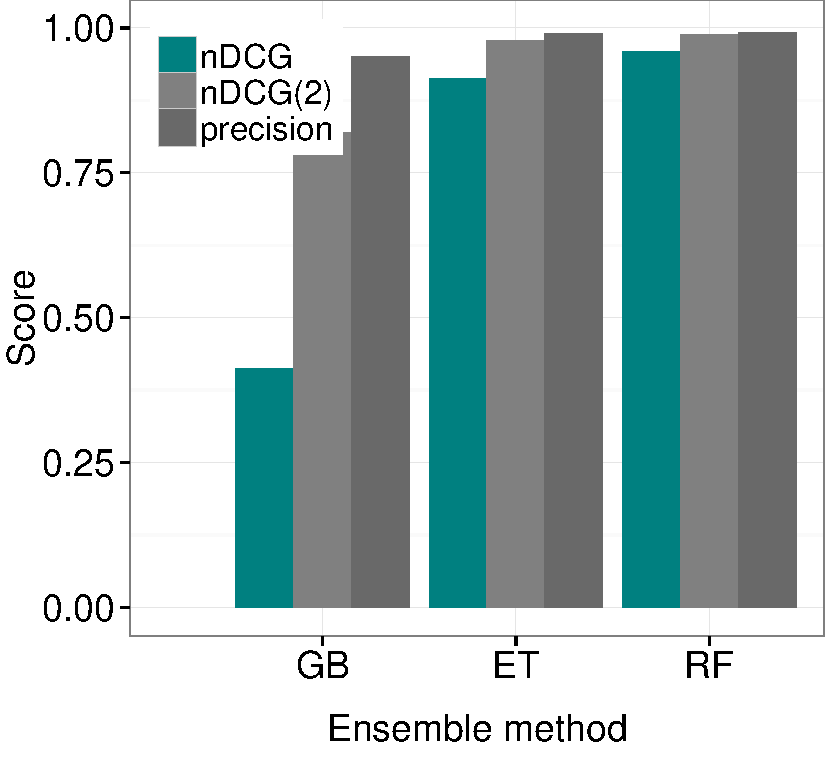
\includegraphics[width=.9\textwidth]{inputs/img/ensemble_method_eval}
		\caption{Ensemble methods evaluation: \textsc{Random Forest}(RF), \textsc{Gradient Tree Boosting}(GB) and \textsc{Extremely Randomized Trees}(ET).}
		\label{fig:ensemble_method_eval}
  %\centering
	\end{minipage}
	\hspace{0.1cm}
	\begin{minipage}[t]{0.48\linewidth}
		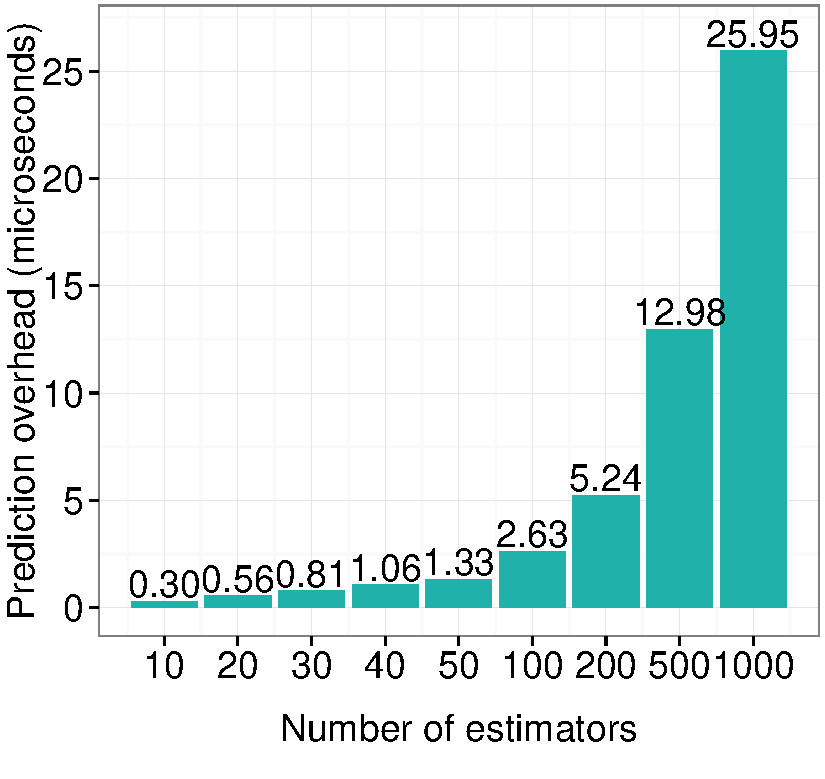
\includegraphics[width=.9\textwidth]{inputs/img/rf_learners}
		\caption{Overhead for different number of estimators of \textsc{Random Forest}.}
		\label{fig:rf_learners}
	\end{minipage}
\end{figure}

\subsubsection{Adjusting the Number of \emph{Estimators} to Learn}

According to Friedman \emph{et al.}, \textsc{Random Forest} performs predictions by building a collection of \emph{de-correlated} trees, namely estimators, and then averages them. We investigated the impact of the number of estimators in ranking accuracy, memory and computation time. We varied the number of estimators progressively from 10 to 1000, with the same previous samples. Results show that the number of estimators has a negligible impact in the accuracy of our model. While a model with 10 estimators scores 0.9594, 1000 scores 0.9569, slightly worse. One reason for this might be the number of inputs, relatively small, that is likely to require a small number of estimators. Yet, the number of estimators impacts on the model overhead, specially for computation time. As depicted in Figure~\ref{fig:rf_learners}, computation time ranges from 0.3 microseconds with 10 estimators to almost 26 microseconds with 1000 ones. Although the worst case still represents low overhead, the lower the better. Memory overhead is rather negligible, ranging from 30 to 32MB. Overall, our model has a quite low overhead, suitable for going online. Since there is no evidence to increase the number of estimators, we keep 10 estimators as a default, fair setting.

\subsubsection{Evaluating Bigger Samples for Fitting the Model}

Towards a higher accuracy, we evaluate bigger samples for fitting the model. We collected more information by running logger simulations. As expected, Figure~\ref{fig:sample_size} confirms that we improve accuracy through bigger samples. The improvement in accuracy was slight, about 0.03 as we use a sample size almost six times bigger, i.e. 683 thousand. It is quite important to highlight, though, that this has no impact on computation time of predictions. Thus, we use the biggest sample for the remaining evaluations.

\begin{figure}[htbp]
	\begin{minipage}[t]{0.48\linewidth}
     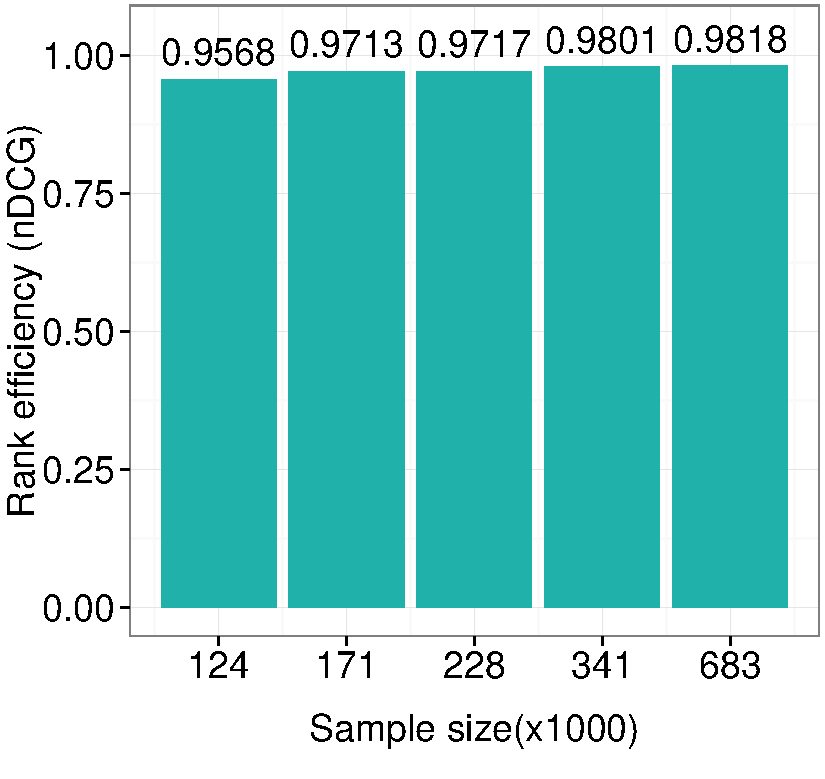
\includegraphics[width=.9\textwidth]{inputs/img/sample_size}
		\caption{Accuracy with different sample sizes.}
		\label{fig:sample_size}
  %\centering
	\end{minipage}
	\hspace{0.1cm}
	\begin{minipage}[t]{0.48\linewidth}
		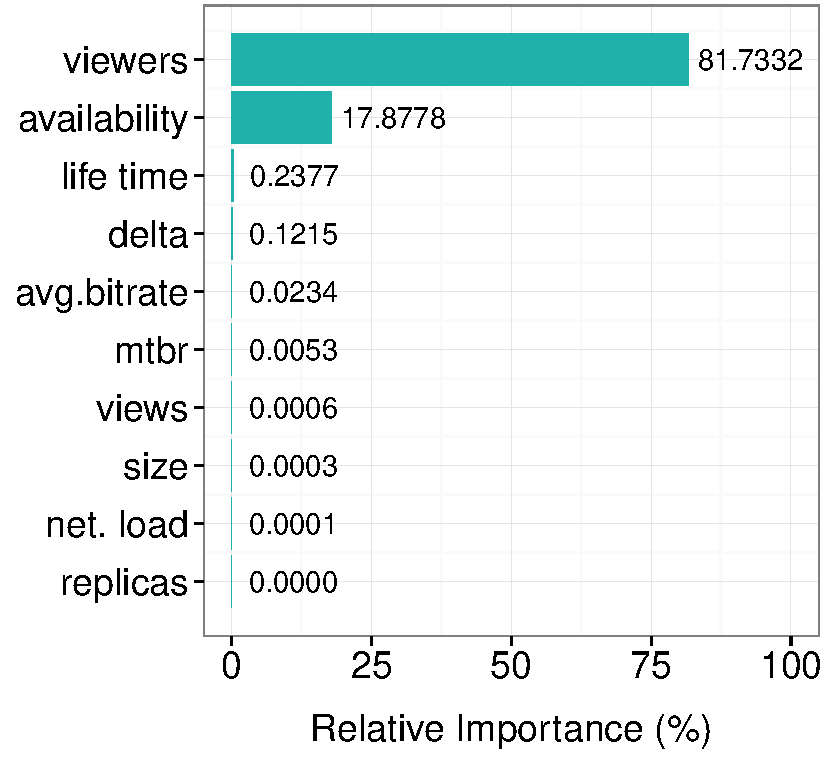
\includegraphics[width=.9\textwidth]{inputs/img/feature_importance}
		\caption{Relative importance to ranking of the 10 model's inputs.}
		\label{fig:feature_importance}
	\end{minipage}
\end{figure}

\subsubsection{Analysing the Relative Importance of Model's Inputs}

We were particularly interested in evaluating the contribution of each input of our model, described in Subsection~\ref{subsec:learning_model_details}. \textsc{Scikit-learn} library allows to measure the relative importance of each input for predicting the ranking position using the \textsc{Random Forest} method. Figure~\ref{fig:feature_importance} highlights the relative importance for all 10 inputs of our ranking model. The two most relevant inputs are the current number of viewers and network availability. These inputs alone account for 99.6\% of the all model's accuracy. It seems quite reasonable, since the former measures the demand for a video and the later depicts the offer of network resources, the main system feature for enforcing average bitrate. The remaining eight inputs are largely irrelevant to the ranking model's accuracy, and may be replaced or removed. Surprisingly, the number of replicas, current network load, and video size seem to be useless to our model. It is likely that network availability is a particularly good measurement, making these eight inputs rather redundant. For simplicity, we include all inputs in the rest of the work. This is harmless for the model's accuracy.

\subsection{Evaluating Replication Strategies in Peer-Assisted VoD Systems}
\label{subsec:performance_evaluation}

In this subsection we analyse the replication strategy used in WiseReplica. First, we evaluate four simple replication policies. Then, we compare WiseReplica with a non-collaborative caching and Oracle-like, all described in Subsection~\ref{subsec:methodology_replication_schemes}. We evaluate their capacity to meet consumers' expectation by observing the number of violations. In addition, we analyse network and storage usage.

\subsubsection{Enforcing Simple Replication Policies on Ranked VoD}

For the three highest rank position, WiseReplica enforces a replica creation policy, described in Subsection\ref{subsec:wisereplica_replication_strategy}. It defines the replication degree growth factor. Considering mean video size of 20MB, we analyse four simple creation policies, namely uniform, linear, quadratic, and exponential.  Table~\ref{tab:creation_policies} show the number of violations by varying $B$ from 2 to 6. Overall, creation policies that take into account the rank positions, i.e. linear, quadratic, and exponential, performed better. Results show that there is relatively small difference for $B\ge 3$, suggesting that our ranking model reacts promptly to modifications on network availability, preventing over-replication. However, for $B\ge 5$, it appears that replication increases the network load system load, causing few more violations. We selected the linear policy with $B=4$ that seems to be the most resilient towards proper resource allocation, providing a fair replication degree growth factor.

\begin{table}
  \label{tab:motivation_advanced_encodings}
	\begin{center}
		\caption{Replication policies.}
  		\label{tab:creation_policies}
		\begin{tabular}{p{1.2cm} || p{1cm} p{1cm} p{1cm} p{1cm} p{1cm}}
		%\begin{tabular}{r||r r r r}
			&\multicolumn{5}{c}{{\bf Parameter $c$}}\\
			{\bf Policy}&{\bf 2}&{\bf 3}&{\bf 4}&{\bf 5}&{\bf 6}\\
			\hline
			\hline
			Uniform&867&567&\cellcolor{blue!25}44&28&23\\
			\cellcolor{blue!25}Linear&\cellcolor{blue!25}123&\cellcolor{blue!25}77&\cellcolor{blue!25}6&\cellcolor{blue!25}9&\cellcolor{blue!25}16\\
			Quadratic&102&21&\cellcolor{blue!25}42&46&58\\
			Exponential&118&32&\cellcolor{blue!25}19&27&28\\
		\end{tabular}
	\end{center}
\end{table}

\subsubsection{Load Resiliency}

A good replication strategy must cope with changes on the system load.  We vary the global load of the system by changing the mean video size, described in Subsection~\ref{subsec:methodology_workload}. Assuming the three mean video sizes 20MB, 30MB and 40MB, caching had 1814, 3864, and 7049 violations respectively, while WiseReplica had only 6, 77, and 106. Figure~\ref{fig:mean_load_bar} compares the number of violations using WiseReplica and a non-collaborative caching. As the load of the system increases, concurrency in bitrate allocation also increases, causing more violations. WiseReplica outperforms caching mostly because it predicts and prevents useless replication. Therefore, we set 40MB as the default mean video size workload setting.

\begin{figure}
  \centering
     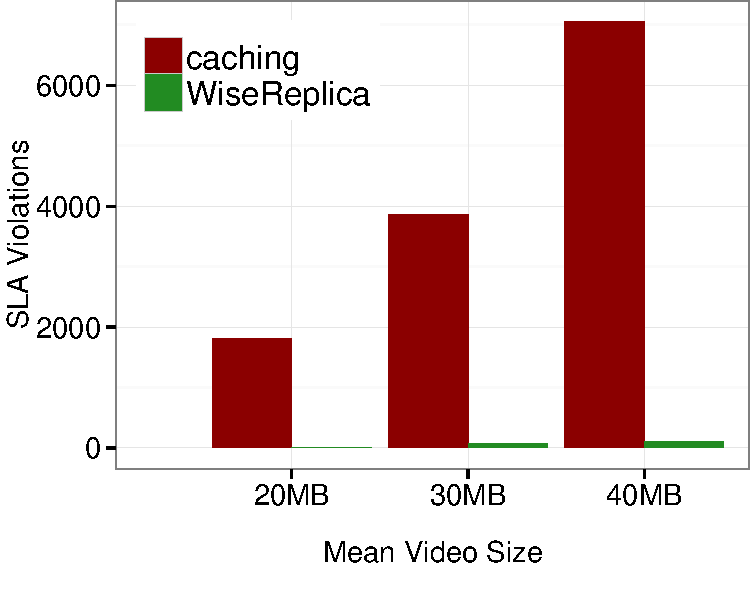
\includegraphics[width=.5\textwidth]{inputs/img/mean_load_bar}
  \caption{Mean Video Size. Higher loads increase the concurrence in network resources, as a result, more violations.}
  \label{fig:mean_load_bar}
\end{figure}

\subsubsection{Benefits of Prediction on Storage Usage}

We aim to adapt the number of replicas to the number of views of a video, especially for the most popular ones. Figure~\ref{fig:replication_for_most_popular} plots the maximum number of replicas for the 1\% most popular videos. Using caching, the maximum number of replicas is high, ranging from 816 to 1367. The Oracle-like assumption allows to decrease significantly the lower and upper limits, to 10 and 190. WiseReplica also reduces the maximum replica range, which is from 19 to 160. More interestingly, the shape of the replication curves of WiseReplica and Oracle-like are quite similar indeed. It confirms that our predictions are accurate, and that a simple replication policy works properly.
% averages cache: 1090, oracle-like: 20, WiseseReplica: 28

Reducing the number of replicas implies that the systems requires less storage for replication. Figure~\ref{fig:cache_usage_for_replication} shows storage usage for replicas by replication scheme. Although WiseReplica utilizes more storage than Oracle-like, its usage remains two orders of magnitude smaller than a non-collaborative caching. The maximum storage usage for Oracle-like, WiseReplica, and a non-collaborative caching were 34, 85, and 7921 GB respectively. WiseReplica creates more replicas than Oracle-like because it does not rely on bandwidth reservation to prevent violations. Despite that, WiseReplica maintains replicas efficiently, keeping storage usage very low, and making cache replacement policies redundant.

\begin{figure}[htbp]
	\begin{minipage}[t]{0.48\linewidth}
		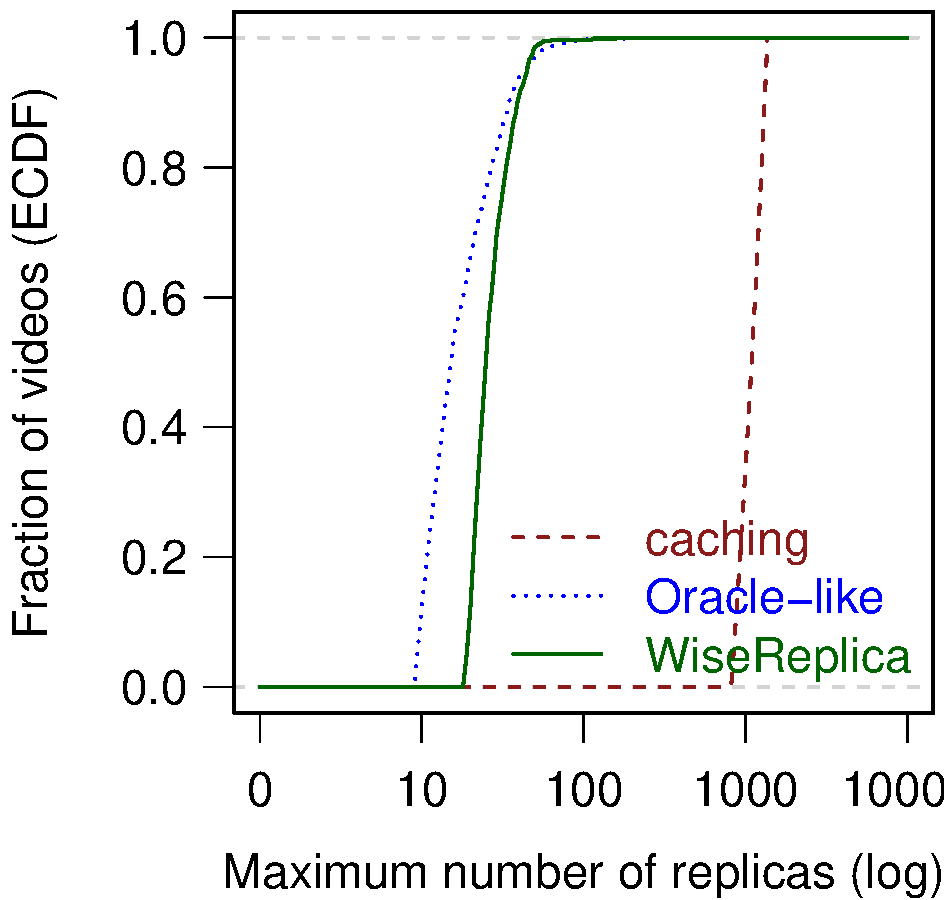
\includegraphics[width=.9\textwidth]{inputs/img/ecdf_replicas}
		\caption{The maximum number of replicas for the 1\% most popular videos.}
		\label{fig:replication_for_most_popular}
  %\centering
	\end{minipage}
	\hspace{0.1cm}
	\begin{minipage}[t]{0.48\linewidth}
     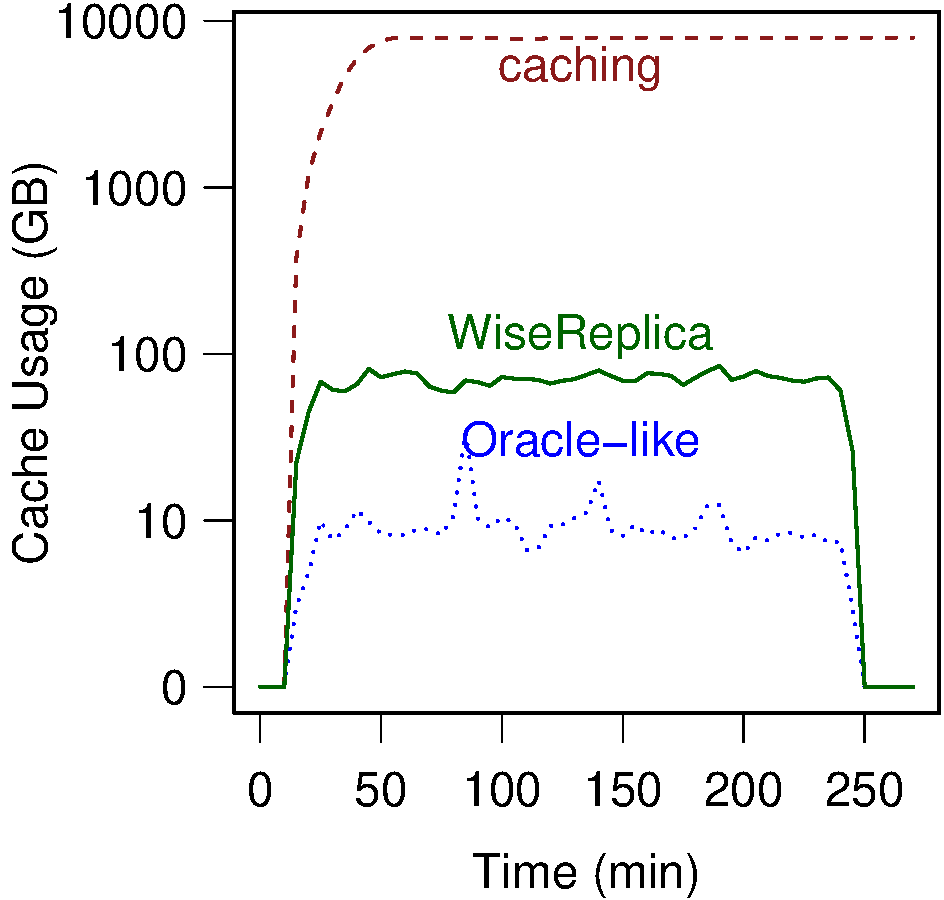
\includegraphics[width=.9\textwidth]{inputs/img/cache_usage}
		\caption{Storage usage for replication.}
		\label{fig:cache_usage_for_replication}
	\end{minipage}
\end{figure}

\subsubsection{Enhancing Bitrate Provision for Meeting Consumers' Expectation}

WiseReplica performance is also quite similar to Oracle-like regarding preventing violations. Each point of the Figure~\ref{fig:violations} represents the number of SLA violations for intervals of five minutes. Overall, caching caused 7049 violations affecting 86\% of all viewers, WiseReplica had just 106 violations, and Oracle-like, evidently, none. Compared to caching, WiseReplica prevents nearly 99\% of violations. It copes with violations by (i) creating new replicas for hot videos only, and (ii) adapting the number of replicas according to the rank position. Vertical lines in Figure~\ref{fig:violations} represent the first access to the 10 videos with the worst content provision through caching. They account for 80.62\% of all caching violations. The appearance of these videos puts the system under heavy load, which makes caching fail to prevent violations.

Figure~\ref{fig:avg_bitrate} depicts the average bitrate for viewers of the 10 videos with the worst content provision using caching. When caching was under heavy load, half of viewers experienced a very low bitrate, ranging between 230Kbps and 2575Kbps. The mean bitrate with caching was 43Mbps. On average, WiseReplica improved this bitrate by roughly 85\% under heavy load. Actually it performs almost as well as the Oracle-like assumption, that improved bitrate provision by 93\%. These finds suggest that WiseReplica largely outperforms caching, fairly meeting consumers' expectations under heavy load conditions.

%\begin{figure}
%  \centering
%     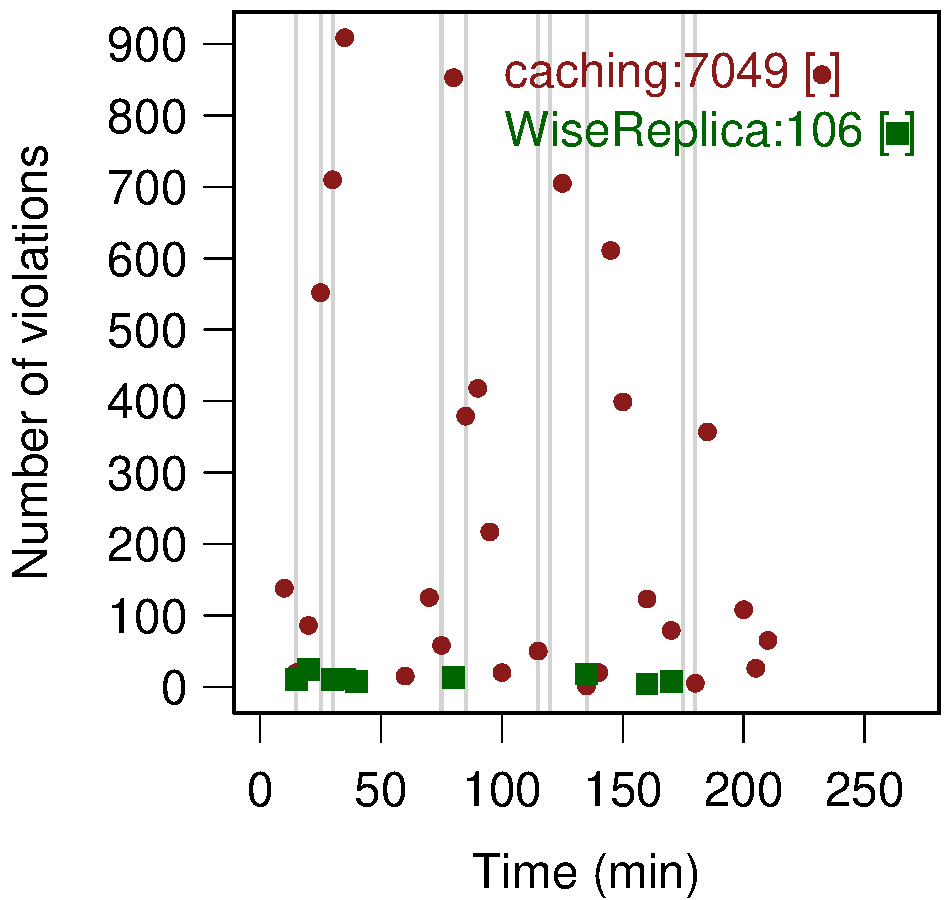
\includegraphics[width=.45\textwidth]{inputs/img/violations}
%  \caption{SLA violations. Vertical lines highlight the first view to 10 videos with the worst content provision using caching.}
%  \label{fig:violations}
%\end{figure}

\begin{figure}[htbp]
  \begin{minipage}[t]{0.48\linewidth}
     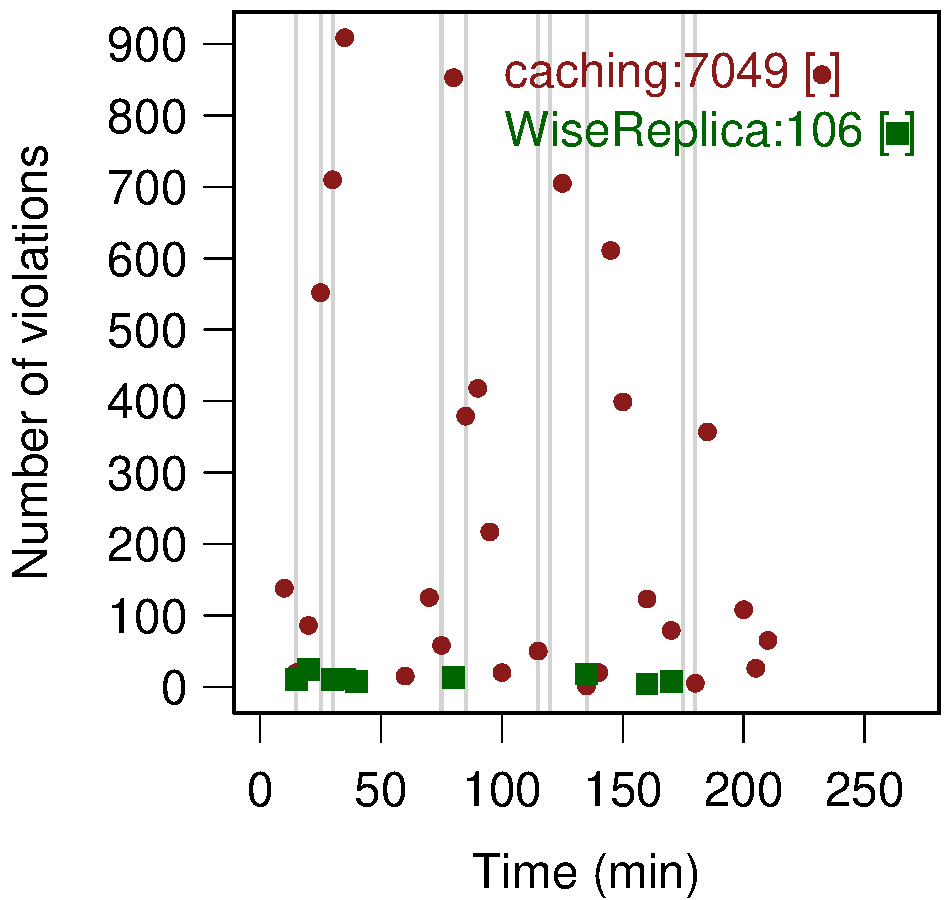
\includegraphics[width=.9\textwidth]{inputs/img/violations}
  \caption{SLA violations. Vertical lines highlight the first view to 10 videos with the worst content provision using caching.}
  \label{fig:violations}
  \end{minipage}
  \hspace{0.1cm}
  \begin{minipage}[t]{0.48\linewidth}
     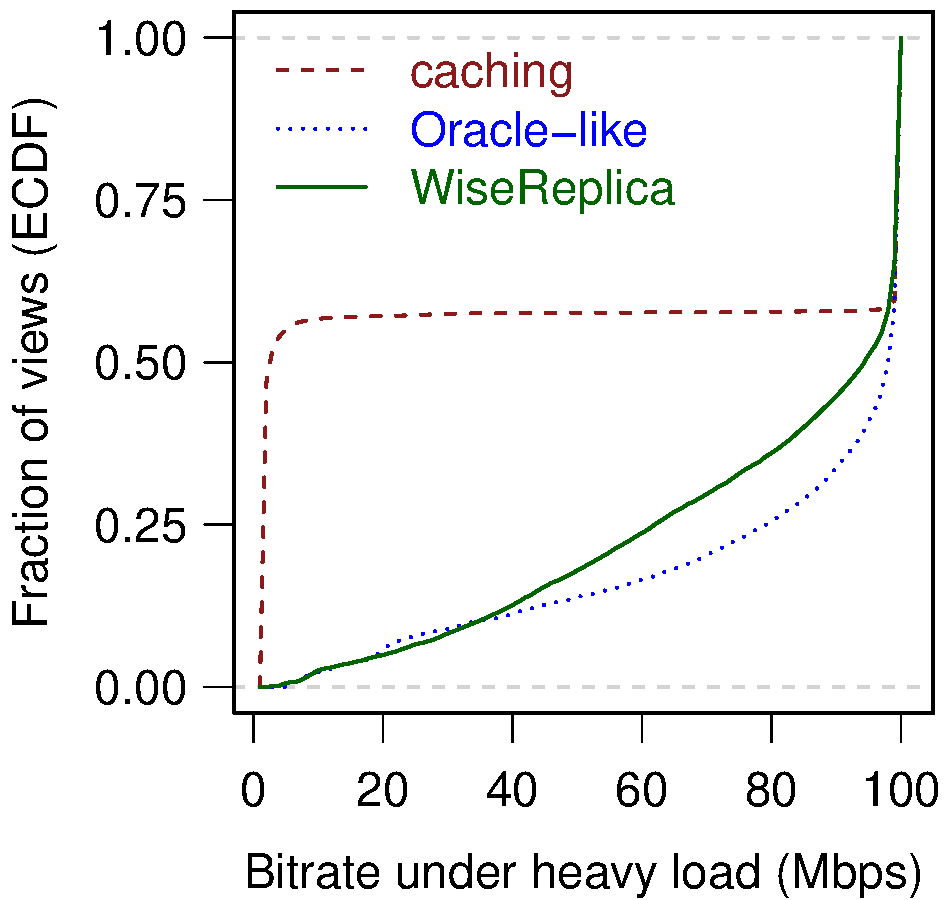
\includegraphics[width=.9\textwidth]{inputs/img/ecdf_agg_bwd_under_heavy_load}
  \caption{Bitrate for viewers of the 10 most popular videos under heavy load.}
  \label{fig:avg_bitrate}
  \end{minipage}
\end{figure}
